\documentclass[11pt,a4paper]{article}

% ============ PAQUETES ============
\usepackage[utf8]{inputenc}
\usepackage[T1]{fontenc}
\usepackage{amsmath, amssymb}
\usepackage{graphicx}
\usepackage{geometry}
\usepackage{tikz}
\usepackage{booktabs}
\usepackage{array}
\usepackage{enumitem}
\usepackage{hyperref}
\usepackage{algorithm}
\usepackage{algpseudocode}
\usepackage{xcolor}
\usepackage{fancyhdr}

% Nota: el paquete babel con el idioma espanol no esta disponible en este
% entorno de compilacion. Se traduce a mano la unica cadena automatica
% que usa este documento ("Resumen").
\renewcommand{\abstractname}{Resumen}

\geometry{margin=2.5cm}
\hypersetup{colorlinks=true, linkcolor=blue, urlcolor=blue, citecolor=blue}

\pagestyle{fancy}
\fancyhf{}
\lhead{Algoritmos Avanzados -- Avance 1}
\rhead{Grupo 1 -- Cobertura de Vértices}
\cfoot{\thepage}

% ============ DATOS DEL PROYECTO ============
\title{
	\vspace{-1.5cm}
	\textbf{Optimización de la Ubicación de Sistemas de Detección de Intrusos \\
	mediante Cobertura de Vértices} \\
	\large Comparación entre heurística greedy por grado y aproximación por emparejamiento maximal
}
\author{
	Grupo 1 \\
	\small Universidad Nacional de San Antonio Abad del Cusco \\
	\small Escuela Profesional de Ingeniería Informática y de Sistemas \\
	\small Asignatura: Algoritmos Avanzados \\
	\small Docente: Héctor Eduardo Ugarte Rojas
}
\date{Semestre académico 2026-2 \\ Avance 1: Formulación y delimitación del problema}

\begin{document}

\maketitle
\thispagestyle{fancy}

\begin{abstract}
\noindent
Este documento presenta la formulación inicial del problema asignado al Grupo~1: la
\textbf{Cobertura de Vértices (Vertex Cover)}, aplicada al contexto de ciberseguridad y
monitoreo de redes. Se especifican las entradas, salidas, restricciones, supuestos y la
función objetivo del problema; se resuelve manualmente una instancia pequeña; se proponen
los algoritmos a implementar y comparar; y se identifican los conocimientos adicionales
que el grupo deberá adquirir de manera autónoma durante el desarrollo del proyecto.
\end{abstract}

% ======================================================
\section{Tema y contexto de aplicación}

El tema asignado al grupo es \textbf{Cobertura de Vértices y comparación de estrategias
de aproximación}. Se abordará dentro del contexto de \textbf{ciberseguridad y monitoreo
de redes}.

En una red de comunicaciones, cada enlace físico entre dispositivos (routers, switches)
constituye un punto potencial de tráfico malicioso o de fallas. Instalar un sistema de
detección de intrusos (IDS) o firewall en \emph{todos} los routers de la red garantiza
visibilidad completa, pero resulta costoso e innecesario. Basta con que cada enlace tenga
\emph{al menos uno} de sus dos extremos monitoreado para poder detectar el tráfico que
circula por él. Este planteamiento corresponde exactamente al problema clásico de
\textbf{Vertex Cover}: encontrar el subconjunto mínimo de vértices tal que toda arista del
grafo tenga al menos un extremo en dicho subconjunto.

\subsection{Motivación}
El problema es relevante porque:
\begin{itemize}[itemsep=2pt]
	\item Minimizar el número de equipos de monitoreo reduce costos de hardware, licencias
	y mantenimiento.
	\item Vertex Cover es un problema NP-difícil clásico con múltiples estrategias de
	solución (exactas, heurísticas y de aproximación con garantía teórica), lo cual permite
	una comparación experimental rica.
	\item Existe una dualidad conocida con el problema de \emph{Independent Set}
	($V \setminus C$ es un conjunto independiente si y solo si $C$ es una cobertura de
	vértices), lo que enriquece el análisis teórico.
\end{itemize}

% ======================================================
\section{Formulación del problema}

\subsection{Modelo}
La topología de la red se representa como un grafo no dirigido $G = (V, E)$, donde:
\begin{itemize}
	\item $V$ es el conjunto de routers/switches de la red.
	\item $E$ es el conjunto de enlaces físicos entre dichos dispositivos.
\end{itemize}

\subsection{Entradas}
\begin{itemize}
	\item Un grafo $G = (V, E)$ que representa la topología de la red.
	\item (Extensión futura) Costo de instalación por nodo, para una variante ponderada
	del problema.
\end{itemize}

\subsection{Salidas}
\begin{itemize}
	\item Un subconjunto $C \subseteq V$: los routers donde se instalará el sistema de
	monitoreo.
	\item El tamaño $|C|$ obtenido por cada algoritmo, para fines comparativos.
	\item Verificación booleana de que $C$ es una cobertura válida de $E$.
\end{itemize}

\subsection{Restricciones}
\begin{itemize}
	\item Para toda arista $(u,v) \in E$ debe cumplirse $u \in C \lor v \in C$.
	\item $C \subseteq V$.
\end{itemize}

\subsection{Supuestos}
\begin{itemize}
	\item La topología de la red es estática durante el cálculo de la solución.
	\item El grafo es no dirigido y no ponderado en esta primera fase del proyecto.
	\item Un router monitoreado detecta el tráfico de \emph{todos} sus enlaces directos.
\end{itemize}

\subsection{Función objetivo}
El problema de decisión/optimización se formula como:
\begin{equation}
	\min_{C \subseteq V} |C|
	\quad \text{sujeto a} \quad
	\forall (u,v) \in E: \; u \in C \; \lor \; v \in C
\end{equation}

Al ser Vertex Cover un problema NP-difícil, no se conoce un algoritmo eficiente que
garantice la solución óptima para instancias grandes, de allí la necesidad de comparar
heurísticas y algoritmos de aproximación frente a una solución exacta de referencia en
instancias pequeñas.

% ======================================================
\section{Instancia pequeña resuelta manualmente}

Se plantea una mini-red de 6 routers como ejemplo ilustrativo:

\begin{center}
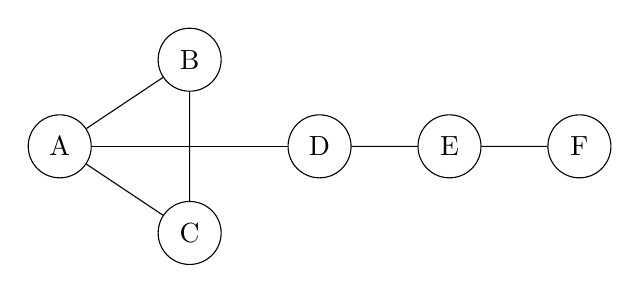
\begin{tikzpicture}[scale=1.1, every node/.style={circle, draw, minimum size=0.8cm}]
	\node (A) at (0,1)   {A};
	\node (B) at (1.5,2) {B};
	\node (C) at (1.5,0) {C};
	\node (D) at (3,1)   {D};
	\node (E) at (4.5,1) {E};
	\node (F) at (6,1)   {F};

	\draw (A) -- (B);
	\draw (A) -- (C);
	\draw (A) -- (D);
	\draw (B) -- (C);
	\draw (D) -- (E);
	\draw (E) -- (F);
\end{tikzpicture}
\end{center}

\textbf{Conjunto de vértices y aristas:}
\[
V = \{A, B, C, D, E, F\}, \qquad
E = \{(A,B),(A,C),(A,D),(B,C),(D,E),(E,F)\}
\]

\textbf{Grados iniciales:} $\deg(A)=3,\ \deg(B)=2,\ \deg(C)=2,\ \deg(D)=2,\ \deg(E)=2,\ \deg(F)=1$.

\subsection{Resolución con Greedy por Grado}
\begin{enumerate}[itemsep=1pt]
	\item Aristas pendientes: $\{AB, AC, AD, BC, DE, EF\}$.
	\item Grado máximo: $A$ (grado 3) $\Rightarrow$ se añade $A$. Se eliminan $AB, AC, AD$.
	\item Pendientes: $\{BC, DE, EF\}$. Grados recalculados: $B{=}1,\ C{=}1,\ D{=}1,\ E{=}2,\ F{=}1$.
	\item Grado máximo: $E$ (grado 2) $\Rightarrow$ se añade $E$. Se eliminan $DE, EF$.
	\item Pendientes: $\{BC\}$. Se elige $B$ (o $C$, indistinto) $\Rightarrow$ se añade $B$.
	\item \textbf{Resultado: } $C_{\text{greedy}} = \{A, E, B\}$, \; $|C_{\text{greedy}}| = 3$.
\end{enumerate}

\subsection{Resolución con Matching Maximal (2-aproximación)}
\begin{enumerate}[itemsep=1pt]
	\item Aristas pendientes: $\{AB, AC, AD, BC, DE, EF\}$.
	\item Se toma arbitrariamente $(A,B)$ $\Rightarrow$ se añaden $A$ y $B$. Se eliminan
	todas las aristas incidentes a $A$ o $B$: $AB, AC, AD, BC$.
	\item Pendientes: $\{DE, EF\}$.
	\item Se toma arbitrariamente $(D,E)$ $\Rightarrow$ se añaden $D$ y $E$. Se elimina
	$EF$ (incidente a $E$).
	\item Pendientes: $\emptyset$ $\Rightarrow$ fin del algoritmo.
	\item \textbf{Resultado: } $C_{\text{match}} = \{A, B, D, E\}$, \; $|C_{\text{match}}| = 4$.
\end{enumerate}

\subsection{Solución óptima de referencia}
Por inspección directa (viable en instancias pequeñas), el conjunto
$C^{*} = \{A, C, E\}$ cubre todas las aristas: $AB$ (por $A$), $AC$ (por $A$ o $C$), $AD$
(por $A$), $BC$ (por $C$), $DE$ (por $E$), $EF$ (por $E$). Por lo tanto
$|C^{*}| = 3$ es \textbf{óptimo}.

\subsection{Observación comparativa}
\begin{center}
\begin{tabular}{lccc}
	\toprule
	\textbf{Algoritmo} & \textbf{Cobertura obtenida} & \textbf{Tamaño} & \textbf{Respecto al óptimo (3)} \\
	\midrule
	Greedy por grado         & $\{A, B, E\}$    & 3 & Óptimo en esta instancia \\
	Matching maximal (2-aprox) & $\{A, B, D, E\}$ & 4 & $1.33\times$ el óptimo \\
	Solución exacta (referencia) & $\{A, C, E\}$ & 3 & --- \\
	\bottomrule
\end{tabular}
\end{center}

En esta instancia particular, el algoritmo greedy alcanza el óptimo mientras que el
matching maximal se aleja ligeramente, aunque siempre dentro de su cota teórica garantizada
de $2\times$ el óptimo. Este tipo de contraste --heurística sin garantía formal pero buen
desempeño práctico vs. aproximación con garantía matemática pero resultado subóptimo en
casos concretos-- es precisamente el eje de la comparación experimental que se desarrollará
en las siguientes entregas.

% ======================================================
\section{Algoritmos propuestos a implementar}

\subsection{Greedy por Grado (\texttt{greedy\_degree\_vertex\_cover})}
Heurística voraz que selecciona iterativamente el vértice de mayor grado respecto a las
aristas aún no cubiertas.

\begin{algorithm}[H]
\caption{Greedy por Grado}
\begin{algorithmic}[1]
\State $\text{remaining\_edges} \gets E$
\State $\text{cover} \gets \emptyset$
\While{$\text{remaining\_edges} \neq \emptyset$}
	\State $v \gets$ vértice con mayor número de aristas incidentes en $\text{remaining\_edges}$
	\State $\text{cover} \gets \text{cover} \cup \{v\}$
	\State eliminar de $\text{remaining\_edges}$ todas las aristas incidentes a $v$
\EndWhile
\State \Return $\text{cover}$
\end{algorithmic}
\end{algorithm}

\noindent \textbf{Complejidad:} $O(|V| \cdot |E|)$ en una implementación directa
(en cada iteración se recorren las aristas restantes para recalcular grados).
\textbf{Garantía:} no tiene una cota de aproximación fija en el peor caso general,
pero exhibe buen desempeño práctico.

\subsection{Matching Maximal / 2-Aproximación (\texttt{maximal\_matching\_vertex\_cover})}
Algoritmo con garantía matemática demostrable: su resultado nunca excede el doble del
tamaño de la cobertura óptima.

\begin{algorithm}[H]
\caption{Matching Maximal (2-aproximación)}
\begin{algorithmic}[1]
\State $\text{remaining\_edges} \gets E$
\State $\text{cover} \gets \emptyset$
\While{$\text{remaining\_edges} \neq \emptyset$}
	\State tomar una arista arbitraria $(u,v) \in \text{remaining\_edges}$
	\State $\text{cover} \gets \text{cover} \cup \{u, v\}$
	\State eliminar de $\text{remaining\_edges}$ todas las aristas incidentes a $u$ o a $v$
\EndWhile
\State \Return $\text{cover}$
\end{algorithmic}
\end{algorithm}

\noindent \textbf{Complejidad:} $O(|V| + |E|)$. \textbf{Garantía:} $|C_{\text{match}}|
\leq 2 \cdot |C^{*}|$, ya que las aristas elegidas forman un \emph{matching} (no comparten
extremos), por lo que cualquier cobertura óptima debe incluir al menos un vértice por cada
arista del matching.

\subsection{Solución exacta de referencia}
Requerida por la guía del proyecto para validar instancias pequeñas. Se propone implementar
una de las siguientes alternativas (a decidir/justificar en la sección de stack tecnológico):
\begin{itemize}
	\item \textbf{Fuerza bruta / branch and bound}: prueba subconjuntos de tamaño creciente
	$k = 1, 2, \dots$ hasta encontrar una cobertura válida, factible solo para $|V|$ pequeño.
	\item \textbf{Programación lineal entera (ILP)}: formulación estándar de Vertex Cover
	resuelta con un solver como \texttt{PuLP} u \texttt{OR-Tools}, propuesta también como la
	tecnología emergente a aprender (indicador AG-C06.02).
\end{itemize}

% ======================================================
\section{Conocimientos adicionales a aprender}

Como parte del plan de aprendizaje autónomo (evidencia del indicador AG-C06.01), el grupo
identifica los siguientes conocimientos que deberá adquirir durante el desarrollo:

\begin{itemize}[itemsep=3pt]
	\item Fundamentos formales de \textbf{NP-completitud} y justificación de por qué
	Vertex Cover pertenece a esta clase.
	\item Demostración formal de la \textbf{garantía de 2-aproximación} del algoritmo de
	matching maximal.
	\item \textbf{Programación lineal entera (ILP)} y uso de un solver
	(\texttt{PuLP} u \texttt{OR-Tools}) como mecanismo de referencia exacto.
	\item Manejo de \textbf{estructuras de grafos en Python} (biblioteca \texttt{NetworkX})
	para representación, manipulación y visualización.
	\item Diseño de \textbf{experimentos reproducibles}: generación de grafos aleatorios y
	de instancias con topología tipo red (p. ej. modelos \emph{Erdős–Rényi},
	\emph{Barabási–Albert} para redes con nodos de alto grado, similares a routers backbone).
	\item Métricas de comparación: ratio de aproximación empírico, tiempo de ejecución y
	escalabilidad frente al tamaño de la instancia.
\end{itemize}

% ======================================================
\section{Conclusiones del avance}

El problema queda formulado como la minimización del número de nodos de monitoreo en una
red modelada como grafo no dirigido, sujeto a que toda arista tenga al menos un extremo
cubierto. Se cuenta con dos algoritmos ya operativos para la comparación
(\texttt{greedy\_degree\_vertex\_cover} y \texttt{maximal\_matching\_vertex\_cover}) y se ha
identificado la necesidad de un tercer componente --una solución exacta de referencia--
para validar resultados en instancias pequeñas, tal como exige la guía del proyecto. La
instancia manual resuelta evidencia que ambos algoritmos son correctos pero pueden diferir
en la calidad de la solución, lo cual sienta las bases para el análisis experimental de las
siguientes entregas.

\end{document}
